\section{Experimental Setup}

\subsection{Simulator and Task}

Experiments use an AutoTrans-like suspended-payload UAV stack in simulation.
The task is to transport a cable-suspended payload to a target under strong
wind while preserving arrival behavior, bounded tracking, and stable
post-arrival hold. The evaluated scenarios focus on Trials 4, 5, and 6, which
were selected in the Stage 4 workflow because they expose strong-wind failures
and method differences.

\subsection{Strict-Valid Metric}

The paper-facing metric is strict-valid count over repeated runs. A
strict-valid run must first satisfy the analyzer-suggested validity field. It
must also have no NaN state, finite maximum swing below 60 deg, finite maximum
UAV and payload speeds below 4 m/s, and final UAV XY error at most 0.5 m.
These stricter checks define success in the protocol-split tables.

We report strict-valid counts rather than only raw suggested validity because
warning-style diagnostics and invalid-only failure groups are needed to
interpret failure modes. Fields such as failure-mode guess, failure group,
command saturation, swing warnings, and
reference/position jump warnings are diagnostic labels. They do not replace
the strict-valid predicate and are not treated as definitive root-cause
attribution.

\subsection{Protocol Definitions}

We evaluate two protocols separately. The single-goal mission protocol uses
goal repeat = 1, meaning the goal is published once. The goal-reissue
stress protocol uses goal repeat = 10, repeatedly republishing the
same goal and stressing reference-update, post-arrival, and repeated-command
behavior.

\begin{figure}[t]
  \centering
  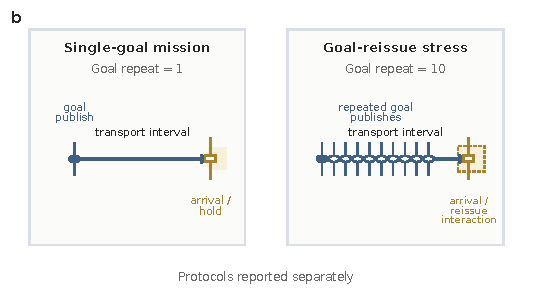
\includegraphics[width=\linewidth]{figures/fig2_protocol_split_nature.pdf}
  \caption{Protocol-split evaluation schematic. The single-goal mission
  protocol uses one goal publish, whereas the goal-reissue stress protocol
  repeatedly republishes the same goal. Results are reported separately; this
  figure defines the protocols and is not a result plot.}
  \label{fig:protocol_split}
\end{figure}

\subsection{Compared Methods}

The complete cross-protocol table includes Original, Fixed Scale 0.85,
Wind-Level 0.85, Fixed Scale 0.80, Risk Adapter v1, and Risk Adapter v2.1.
Risk Adapter v2 has a single-goal result but lacks the matching stress result,
so it is treated as a supplementary single-protocol-only note rather than a
main balanced-ranking entry.

\subsection{Repeated-Run Design and Diagnostic Logging}

Each complete method/protocol combination is evaluated over 30 repeated runs
across Trials 4, 5, and 6. Diagnostic logs support strict-valid classification,
invalid-only failure grouping, command-scale inspection, warning-score
inspection, arrival timing, NaN timing, and representative trace analysis. These diagnostic
views are used to interpret failures, not to replace strict-valid count as the
main paper metric.
